\section{Today's assignment}
Today's class will demystify the Transformer architecture \cite{vaswani2017attention}. Transformers have become the dominant model in Natural Language Processing pushing the performance of all tasks through models like BERT \cite{devlin2018bert} and GPT \cite{brown2020language}. In this class, we will review the architecture of Transformers. The focus of the class is to understand and implement the self-attention mechanism in Pytorch. For this, we will use an annotated version of Karpathy's miniGPT library.


\section{Before Diving into Transformers}
Before diving into transformers, we would like to introduce two important pieces of details to defining and training transformers.


\subsection{Positional Encoding}
Different from models with recurrence/convolution, positional information is not encoded in Transformers. Therefore, \citet{vaswani2017attention} include the positional embedding as part of the input to Transformers. The most popular way to compute the positional embedding ($PE$) is to use the sinusoidal expressed as
\begin{equation}
        PE_{(pos,2i)} = sin(\frac{pos}{ 10000^{2i/d_{model}}}),
\end{equation}
\begin{equation}
    PE_{(pos,2i+1)} = cos(\frac{pos}{ 10000^{2i/d_{model}}}),
\end{equation}

where $pos$ is the position and $i$ is the dimension.

\subsection{Tokenization}
Transformers are trained with the byte pair encoding \citep{bpe} approach for tokenizing text sequences, enabling encoding rare and unknown words as sequences of subword units.

\begin{exercise}
Tokenization
\begin{enumerate}
\item Run the word-based tokenizer and try out different{\tt text}:
\begin{python}
text = "I travelled to Lisbon in July to attend an NLP summer school"
text.split()
\end{python}
\item Run the character-based tokenizer, try out different different{\tt text} and answer the corresponding question:
\begin{python}
text = "I will travel to Lisbon in July..."
tokenized = [c for c in text if c not in [",", ";", ":", "'", "!", "?"]]
print(tokenized)
\end{python}
\item Run the BPE (byte-pair encoding) tokenizer, and answer corresponding questions:
\begin{python}
import numpy as np
from lxmls.transformers.bpe import BPETokenizer

tokenizer = BPETokenizer()

sentence = "Your drawing is charmingly anachronistic."
tokenizer.encoder.encode_and_show_work(sentence)
\end{python}
\end{enumerate}
\end{exercise}
\section{Transformer Architectures}

The basic building block of the Transformer combines a large Feed forward network with a multi-head self-attention layer. We have seen feed forwards in previous days and we will focus here on multi-head self-attention. Refer to previous days for details on the basics of feed-forwards.

Transformer blocks can be found in three types: Encoder, Decoder, and Encoder-Decoder 

\begin{enumerate}
\item Encoders: map a sequence of $T$ observations, e.g. some word or sub-word units $x_1 \cdots x_T$ to a hidden representation of size $H$, yielding a matrix of embeddings of size $(H, T)$. These contextual embeddings can be used to build other models on top by adding extra layers e.g. BERT.
\item Decoders: given a sequence of $t$ observations, e.g. some word or sub-word units $x_{<t} = x_1 \cdots x_{t-1}$ provide a hidden representation for element $x_t$. This can be used to predict the next word given some partial sentence e.g. as in GPT. 
\item Cross-Attention-Decoders: map a sequence $x$ to another of different size $y$. For this, they first Encode $x$ using an encoder. And then use a modified Decoder, that uses an additional attention mechanism read the Encoder values to generate embeddings for $y_t$ given $y_{<t}$ and the $\mathrm{Encoder}(x)$. The original Transformer used for machine translation is the best example.
\end{enumerate}

Though with very different roles the three architectures are very close to each other and imply only minor modifications. We will focus here on the Encoder architecture first, and then we will explain the other two.

\section{Attention}
In this section, we will delve into the intricacies of the attention mechanism, aiming to grasp its underlying intuition and motivation. We will embark on a comprehensive exploration of its inner workings, unraveling its secrets along the way.

Attention mechanisms have become a crucial component in effective sequence modeling across different tasks e.g. Neural Machine Translation (NMT) \cite{vaswani2017attention}. They enable the modeling of relationships between elements in input or output sequences, regardless of their positional distance. \cite{bahdanau2014neural, kim2017structured}.

The state-of-the-art sequence modeling architectures that predate Transformers, such as Recurrent Neural Networks (RNN), have traditionally treated input information in a uniform manner. This means that no specific connections are established among the individual tokens to fully capture the intricate relationships between them. Essentially, each token denoted as $t_i$, receives information from all preceding tokens $t_1...t_{i-1}$ in a uniform fashion. However, as the value of $i$ increases, this approach often leads to information loss, as well as issues related to vanishing or exploding gradients \cite{hochreiter1997long}, due to the fixed dimensionality of the encoded information.

In order to mitigate the latter challenge, Long Short-Term Memory (LSTM) models were introduced. These models proposed mechanisms to manipulate the flow of information across states by selectively adding or removing pertinent and extraneous information \cite{hochreiter1997long}. By incorporating these mechanisms, LSTM models aimed to address the aforementioned issues and enhance the handling of information within the sequence.
The LSTM has demonstrated exceptional performance on challenging sequence prediction tasks, such as text translation, and swiftly emerged as the prevailing approach in the field \cite{cho2014learning, sutskever2014sequence}.

However, the issue of having a fixed-length internal representation persists, and to overcome this limitation in the encoder-decoder architecture, the Attention mechanism was introduced. The Attention mechanism offers various variants, and in this context, we will delve into the "Scaled Dot-Product Attention" as outlined in \cite{vaswani2017attention}.

To provide a practical demonstration of the complex relationships that the model needs to learn, let's consider the following example: \emph{``The cat didn't climb the tree because it was too scared.``}.
\begin{figure}[h]
    \centering
    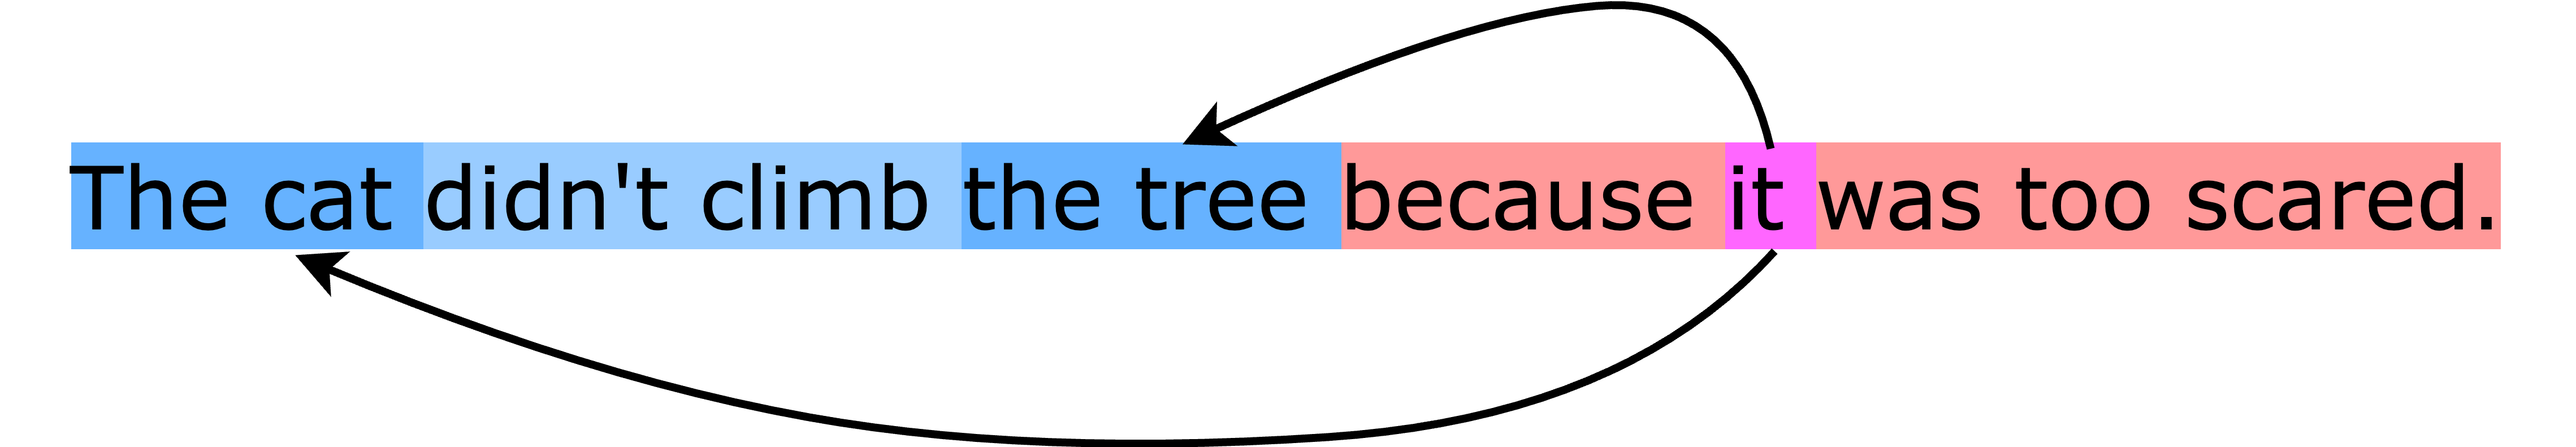
\includegraphics[width=8cm]{pages/imgs/example.png}
    \caption{An example illustration}
    \label{fig:example}
\end{figure}
In the initial part of the example, the inner connections are relatively straightforward. However, in the subsequent segment starting from the word "because," the relationships become more intricate.
For a human being, the question of whether the pronoun "it" refers to the cat or the tree is relatively simple due to our prior knowledge about cats and trees. With our understanding of these concepts, we can confidently determine the intended reference of the word "it." 
However, for a model, discerning the referent of the pronoun "it" -- whether it pertains to the cat or the tree -- is not as straightforward. Therefore, we require a mechanism that does not treat all words with equal importance but rather allocates focus to different tokens.

This intuitive mechanism is known as Attention, which assigns significance to specific tokens for a selected token. In Figure \ref{fig:att_self_sample}, the attention mapping of our example is demonstrated. This is commonly referred to as Self-Attention, as the connections are attained at the internal level, i.e. between input tokens.

\begin{figure}[h]
    \centering
    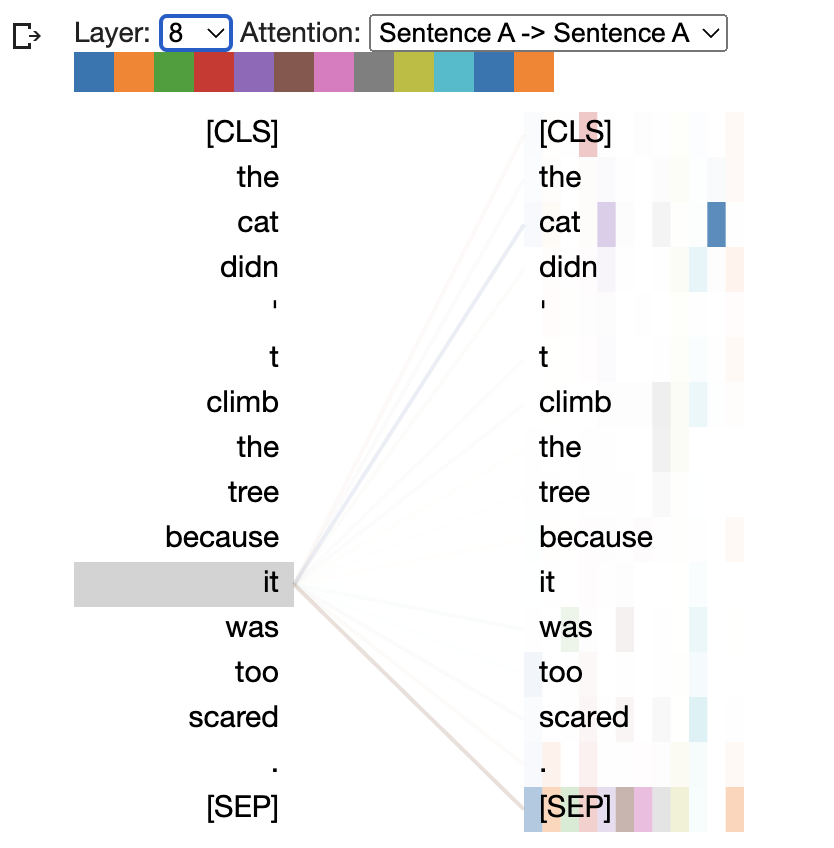
\includegraphics[width=8cm]{pages/imgs/att_self_sample.png}
    \caption{Self-Attention of the sample}
    \label{fig:att_self_sample}
\end{figure}

Capturing the connections between an input and an output sequence is vital for downstream tasks, like Neural Machine Translation (NMT). In this case, the Encoder-Decoder attention mechanism operates in a manner similar to Self-Attention. Let's translate our sample sentence into Portuguese and explore the significant connections it reveals. To accomplish this, we will utilize a pre-trained language model called Multilingual BERT (mBERT), which has knowledge about multiple languages, including English and Portuguese \cite{devlin2018bert}.


\begin{figure}[h]
    \centering
    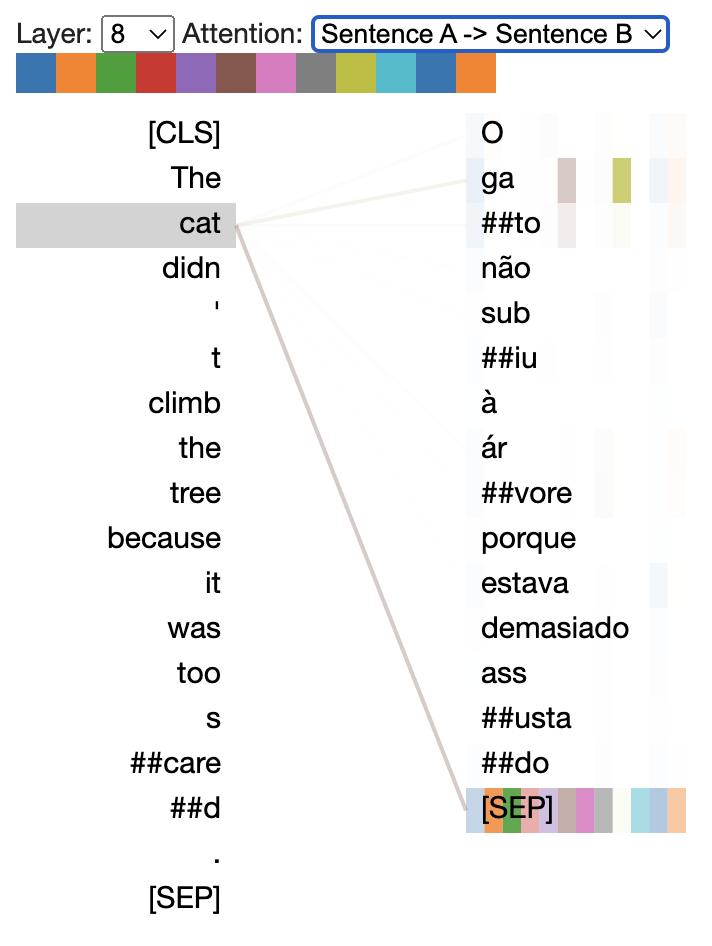
\includegraphics[width=8cm]{pages/imgs/att_cat_sample.png}
    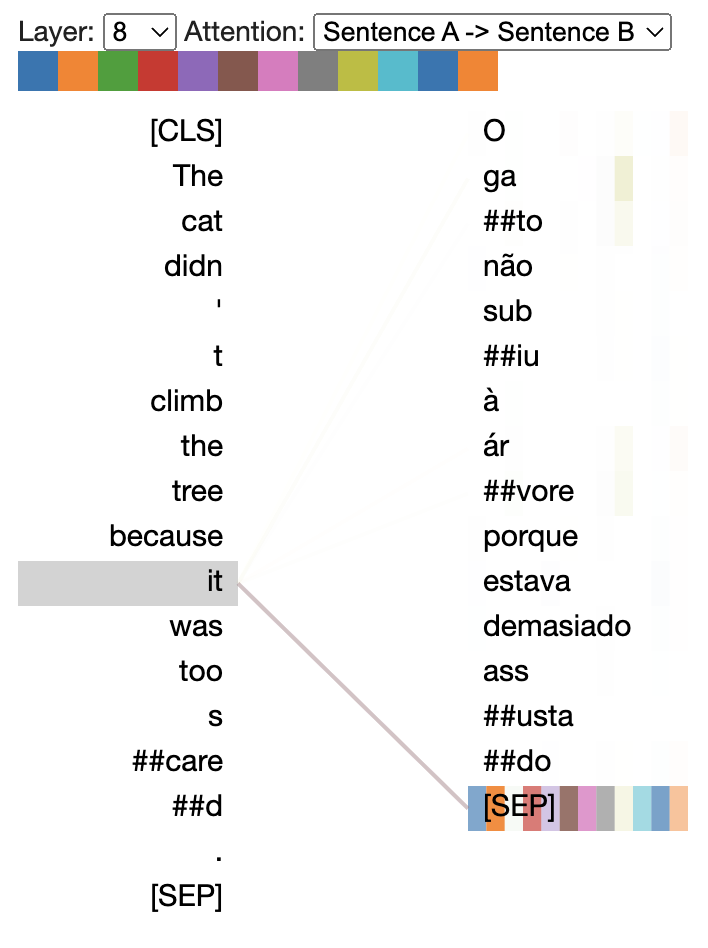
\includegraphics[width=8cm]{pages/imgs/att_it_sample.png}
    \caption{Encoder-Decoder Attention of the sample}
    \label{fig:ed_att_sample}
\end{figure}

In the left image of Figure \ref{fig:ed_att_sample}, we can clearly see that the attention of the token 'cat' is specifically directed towards the token 'gato,' which corresponds to its accurate translation. Similarly, in the right image, the word 'it' is attentively aligned with the token 'gato' once again. These observations indicate the system's ability to effectively focus on the appropriate tokens, both in correctly selecting the appropriate translation, and accurately identifying the relevant noun.

Now let's explore each building block of the Transformer architecture and examine how the Attention mechanism fits in this.



\section{Encoder Architecture}\label{sec:enc}

In the original paper for transformers \citep{vaswani2017attention}, a ``sub-layer`` is formed by either a Feed-Forward ($\mathrm{FF}$) or Multi-Head Attention $\mathrm{MHA}$ (or other named $\mathrm{sub-block}$s) followed by a sequence of operations. In this section, we begin by explaining the encoder architecture. Note that the notation of ``sub-layer`` also applies to the following sections.

\subsection{Simplified Encoder Architecture}

the encoder architecture can be succinctly described as stacking a number of $N$ blocks on top of each other combining a $\mathrm{FF}$ and $\mathrm{MHA}$ sub-blocks. A single block is defined as

\begin{equation}
e^{n+1} = \mathrm{FF}(\mathrm(MHA(e^n)).
\end{equation}

The input to the first block $e^0$ is the sum of position $P$ and non-contextual embeddings $E$ of the input. Assuming $x_1 \cdots x_T$ is a sequence of integers (indices to a vocabulary of $V$ symbols) we have that

\begin{equation}
e^{0}_t = \mathrm{E} \cdot \mathrm{1}_{x_t} + \mathrm{P} \cdot \mathrm{1}_t \quad \mbox{for} \quad t=1 \cdots T
\end{equation}

where $\mathrm{1}_{x_t}$ and $\mathrm{1}_t$ are indicators, i.e. one-hot, vectors for the token content (vocabulary symbol) and the token position. $\mathrm{E} \in \mathbb{R}^{H \times V}$ is the non-contextual embedding matrix for each symbol in the vocabulary and $P^{H \times \tau}$ is the position embedding matrix, where  $\tau-1$ is the furthest position supported. See Figure \ref{fig:e0} for information flow. \\


\begin{figure}[h]
    \centering
    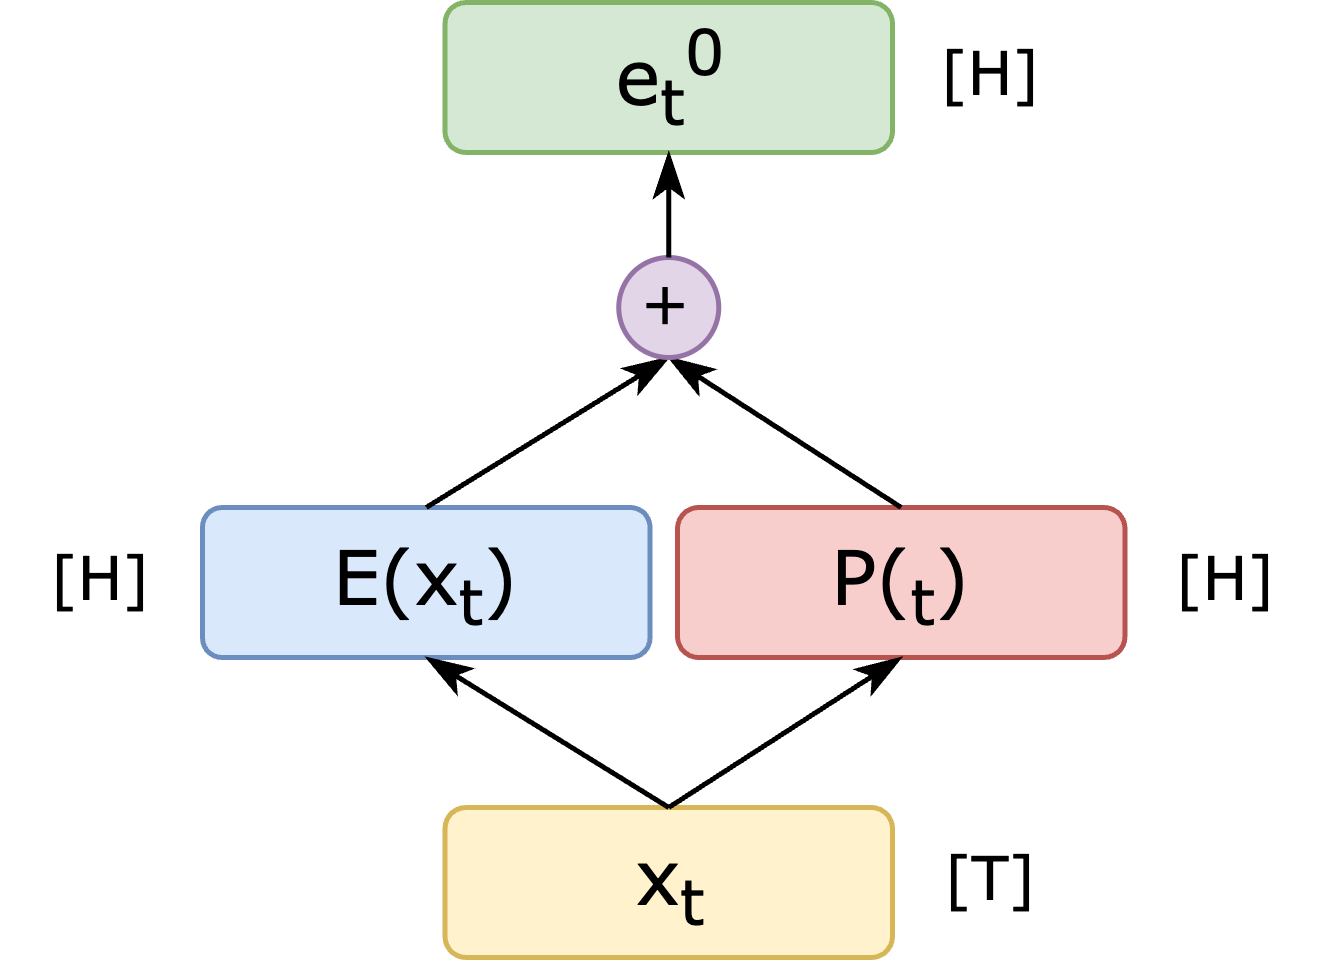
\includegraphics[width=6cm]{pages/imgs/e0.png}
    \caption{Information flow of $t$-th token in layer $e^0$}
    \label{fig:e0}
\end{figure}



\noindent The feed-forward ($\mathrm{FF}$) is given by:

\begin{equation}
FF(z) = W^2\cdot \mathrm{gelu}(W^1 \cdot z)
\end{equation}

\noindent with weight matrices $W^2 \in \mathbb{R}^{H \times 4H}$ and $W^1 \in \mathbb{R}^{4H \times H}$, that expand and contract the hidden dimension $H$.

The Self-Attention ($\mathrm{SA}$) comprises three matrices extracted from the encoder’s input $z$. So, for every given input $z$, we generate a Key vector($K$), a Query vector($Q$), and a Value vector($V$). These matrices are obtained by performing matrix multiplication between the embedding and the corresponding matrix that was learned in the training process, e.g. $Q = W^Q z$.

The next step is to calculate the self-attention score. The Key and Query matrices are multiplied by each other and normalized by a constant value $\frac{1}{A} \left(W^K z\right)^T W^Q z$ or $\frac{1}{A} K^T Q$. The $A$ is usually chosen to be the square root of the dimension of the key matrices. This leads to having more stable gradients.

\noindent Then pass the result through a $softmax$ operation. The Softmax normalizes the scores so they’re all positive and add up to 1. In other words, extracts a distribution of relative scores from a given token for each token in the input sequence.

\noindent After this multiply the output by the Value matrix: $W^V \cdot z \cdot \underset{i \rightarrow}{\mathrm{softmax}}\left( \frac{1}{A} \left(W^K z\right)^T W^Q z \right)$ or simply $V \cdot \underset{i \rightarrow}{\mathrm{softmax}}\left( \frac{1}{A} \left(K \right)^T Q \right)$.

The Multi-Head Attention ($\mathrm{MHA}$) enhances the Self-Attention layer in two ways: it allows the model to focus on different positions within the input, enabling a better understanding of pronoun references; and allowing projection of input embeddings into distinct representation subspaces, thereby improving overall performance.

\noindent Finally getting the following mathematical form for the $\mathrm{MHA}$:


\begin{equation}
MHA(z) =  W^o \cdot
\begin{bmatrix}
    W^V_1 \cdot z \cdot \underset{i \rightarrow}{\mathrm{softmax}}\left( \frac{1}{A} \left(W^K_1 z\right)^T W^Q_1 z \right)\\
    W^V_2 \cdot z \cdot \underset{i \rightarrow}{\mathrm{softmax}}\left( \frac{1}{A} \left(W^K_2 z\right)^T W^Q_2 z \right)\\
    \cdots\\
    W^V_D \cdot z \cdot \underset{i \rightarrow}{\mathrm{softmax}}\left( \frac{1}{A} \left(W^K_D z\right)^T W^Q_D z \right)\\
\end{bmatrix}\nonumber
\end{equation}

where we have $D$ attention heads. Each head contracts the hidden dimension $W^K, W^Q, W^V \in \mathbb{R}^{H / D \times H}$ into a space of size $H / D$ (this has practical implementation consequences). Outputs of all heads are concatenated and projected again with $W^o \in \mathbb{R}^{H \times H}$.

\subsection{Adding Dropout, Residuals, and Layer Normalization}

%For simplicity, we have left several additional operations that can be added as a wrapper around $\mathrm{FF}$ and $\mathrm{MHA}$ operations. These can be expressed as

%\begin{equation}
%C(f)(x) = x + \mathrm{dropout}(f(\mathrm{layernorm}(x)))
%\end{equation}

%where $f = \{\mathrm{FF}, \mathrm{MHA}\}$.

To complete the ``sub-layer``, an dropout followed by a residual connection and a layer normalization is applied to input $z$ that has been passed through a $\mathrm{sub-block}$, where a $\mathrm{sub-block} \in \{\mathrm{FF}, MHA\}$. Together, we can express the function as

\begin{equation}
C(x) = \mathrm{layernorm}(\mathrm{residual}(\mathrm{dropout}(\mathrm{sublayer}(z)), z)
\end{equation}

where $\mathrm{sublayer} \in \{\mathrm{FF}, \mathrm{MHA}\}$.


Specifically, we have
\begin{itemize}
    \item $\mathrm{dropout}(x) = r * x$ where $ r_j \sim \operatorname{Bernoulli}(p)$ and $*$ refers to element-wise multiplication\footnote{Note that the default $p$ is $0.1$.},
    \item $\mathrm{residual}(x, z) = x + z$, and 
    \item $\mathrm{layernorm}(x) = \frac{x-E(x)}{\sqrt{Var(x)+\epsilon}}*\gamma + \beta$ where $E(x)$ and $Var(x)$ are computed among dimensions other than the dimension for the batch\footnote{Note that the default $\epsilon$ is $1e-5$. $\gamma$ and $\beta$ are learnable affine parameters if we want to learn, otherwise set to $1$ and $0$}.
\end{itemize}


\section{Decoder Architecture}\label{sec:dec}

This is identical to the Encoder architecture with two differences

\begin{enumerate}
    \item We feed if a partial sequence $x_{<t}$ and take the last output $h_{t-1}$ as the hidden vector for $x_t$
    \item We mask every head of $\mathrm{MHA}$ to prevent any value of time $p$ to depend on values of $>p$
\end{enumerate}

The implementation of training realizes 1) by masking input partial sequence $x_{<t}$ and hidden units from the corresponding positions with an attention mask. This attention mask is also applied during inference time. 

\section{Encoder-Decoder Architecture}

In the Encoder-Decoder Architecture, the encoder is the same as section \ref{sec:enc}. Therefore, we have the encoded embeddings as $e^N = \mathrm{Encoder}(x)$.

The decoder in the Encoder-Decoder Architecture is a little bit different than section \ref{sec:dec}. Each layer of the decoder will include one more Cross-Multi-Head Attention (CMHA) sub-layer, and the order of sub-layers in a decoder layer will be $\mathrm{MHA}$-$\mathrm{CMHA}$-$\mathrm{FF}$, i.e.

\begin{equation}
    d^{m+1} = \mathrm{FF}(\mathrm(CMHA(e^N, MHA(d^m))).
\end{equation}

Specifically, the query matrix is computed from the layer below it, while the key and value matrix are computed from $e^N$, which can be expressed as

\begin{equation}
    \mathrm{CMHA}(e^N, MHA(d^m)) = W^o \cdot
\begin{bmatrix}
    W^V_1 \cdot e^N \cdot \underset{i \rightarrow}{\mathrm{softmax}}\left( \frac{1}{A} \left(W^K_1 e^N\right)^T W^Q_1 MHA(d^m) \right)\\
    W^V_2 \cdot e^N \cdot \underset{i \rightarrow}{\mathrm{softmax}}\left( \frac{1}{A} \left(W^K_2 e^N\right)^T W^Q_2 MHA(d^m) \right)\\
    \cdots\\
    W^V_D \cdot e^N \cdot \underset{i \rightarrow}{\mathrm{softmax}}\left( \frac{1}{A} \left(W^K_D e^N\right)^T W^Q_D MHA(d^m) \right)\\
\end{bmatrix}\nonumber.
\end{equation}

\begin{exercise} 
Cross Multi Head Attention \& Multi Head Attention
\begin{enumerate}
\item Complete the {\tt cross\_attention} function:
\begin{python}
import torch
import torch.nn.functional as F

def cross_attention(S1, S2, W_Q, W_K, W_V):
    ## Your code here
    return attended_values
\end{python}
\item Complete the {\tt CausalSelfAttention} class. First, you should create linear projections {\tt query\_proj}, {\tt key\_proj} and {\tt value\_proj}.
\begin{python}
import math
import torch.nn as nn

class CausalSelfAttention(nn.Module):

    def __init__(self, config):
        super().__init__()
        
        # Initialize layers and parameters
        self.hidden_size = config.n_embd
        self.num_heads = config.n_head

        # TODO: Create the linear projections

        self.output_proj = nn.Linear(config.n_embd, config.n_embd)

        self.attn_dropout = nn.Dropout(config.attn_pdrop)
        self.resid_dropout = nn.Dropout(config.resid_pdrop)

        self.register_buffer(
            "bias",
            torch.tril(torch.ones(config.block_size, config.block_size)).view(
                1, 1, config.block_size, config.block_size))
\end{python}
Then apply {\tt query\_proj}, {\tt key\_proj} and {\tt value\_proj} to split input into query, key, and value tensors:
\begin{python}
    def forward(self, x: torch.Tensor) -> torch.Tensor:
        B, T, C = x.size()

        # TODO: Split input into query, key, and value tensors

        # Reshape and transpose tensors for multi-head computation
        query = query.view(B, T, self.num_heads,
                           self.hidden_size // self.num_heads).transpose(1, 2)
        key = key.view(B, T, self.num_heads,
                       self.hidden_size // self.num_heads).transpose(1, 2)
        value = value.view(B, T, self.num_heads,
                           self.hidden_size // self.num_heads).transpose(1, 2)
\end{python}
Then compute the attention scores. Note that the shape of scores should be {\tt (B, num\_heads, T, T)}
\begin{python}
        # TODO: Compute attention scores

        # Apply causal mask to restrict attention to the left in the input sequence
        mask = self.bias[:, :, :T, :T]
        scores = scores.masked_fill(mask == 0, float('-inf'))
\end{python}
Finally, apply soft-max activation and multiply attention weights with values to get attended values:
\begin{python}
        # TODO: Apply softmax activation to get attention weights

        # TODO: Multiply attention weights with values to get attended values

        # Transpose and reshape attended values to restore original shape
        attended_values = attended_values.transpose(1, 2).contiguous().view(
            B, T, C)

        # Apply output projection and dropout
        output = self.resid_dropout(self.output_proj(attended_values))

        return output
\end{python}
\end{enumerate}
\end{exercise}

\section{Training different Transformers}
We have introduced different architectures of transformers, and will introduce different variants of transformers that are trained with different objectives, thus applied to different downstream tasks. We provide a brief introduction to all these transformers, and provide the references so you can read these papers if you are interested.

\subsection{Training with Encoders}
Encoder models solely utilize the encoder component of a Transformer model. In each step, the attention layers have the ability to consider all the words present in the original sentence. These models are known as 'auto-encoding models' and are recognized for their 'bi-directional' attention mechanism.

The pretraining of these models typically involves manipulating a given sentence, often by obscuring random words within it and assigning the model the task of identifying or reconstructing the original sentence. This objective is commonly referred to as Masked Language Modeling (MLM), and models pre-trained with this objective are known as Masked Language Models.

Encoder models excel in tasks that demand a comprehensive understanding of the entire sentence. These tasks include sentence classification, word classification tasks e.g. named entity recognition, as well as extractive question answering. Widely used representatives of this model family include BERT \cite{devlin2018bert} and RoBERTa \cite{liu2019roberta}.

\textbf{BERT} \cite{devlin2018bert} is trained on MLM(Masked Language Modeling) and NSP(Next Sentence Prediction) objectives.
In the \textbf{MLM} objective, 15\% of the input tokens are selected. Among these selected tokens:
\begin{itemize}
    \item 80\% of the time, the mask token is inserted in place of the original token.
    \item 10\% of the time, a random token is inserted in place of the original token.
    \item 10\% of the time, the original token remains unchanged.
\end{itemize}
The \textbf{NSP} objective is applied to pairs of sentences, A and B, taken from the training set. In 50\% of the cases, sentence B directly follows sentence A in the input, while in other cases, the pairs are randomly selected. The objective is to perform binary classification and predict whether sentence B follows sentence A or not.

\textbf{RoBERTa} \cite{liu2019roberta} builds upon BERT's pre-training by addressing its perceived undertraining. It introduces the following modifications:
\begin{itemize}
    \item Longer and larger-scale training: RoBERTa trains the model for an extended period using larger batches, more data, and longer sequences.
    \item Removal of NSP objective: The next sentence prediction (NSP) objective, present in BERT, is eliminated in RoBERTa.
    \item Dynamic masking: RoBERTa employs dynamic masking by duplicating the training data ten times and applying different mask patterns to each sample. This contrasts with BERT's static masking, where a fixed mask is used for each sample.
\end{itemize}
These modifications aim to enhance RoBERTa's pre-training performance and overall language understanding capabilities.




\subsection{Training with Decoders}
\paragraph{GPTs.} The class of GPTs are a series of pretained decoder-only transformers. Models are pre-trained to perform next token prediction with Cross-Entropy criterion. Since the release of GPT-1 \citep{gpt-1}, GPTs are being trained with more parameters and training data, with GPT-2 \citep{gpt-2}, GPT-3 
\citep{gpt-3}, InstructGPT \citep{instructgpt} and GPT-4 \citep{gpt-4} being subsequently released. Note that since the release of InstructGPT \citep{instructgpt}, this class of language models have been trained with reinforcement learning with human feedback \citep{rlhf}, which enables the model to manifest interesting behaviors that you see when using ChatGPT.
\subsection{Training with Encoder-Decoder}
\paragraph{BART.} BART \cite{lewis-etal-2020-bart} an encoder-decoder model pre-trained on five tasks injecting noises into the input text: i) token masking (same as BERT \cite{devlin2018bert}), ii) token deletion, iii) text infilling by replacing sampled input spans with single masks, iv) sentence permutation, and v) document rotation. The powerful pre-trained denoising autoencoder is commonly used in generation tasks.
\paragraph{T5.} TODO


\begin{exercise}
Training Transformer
\begin{enumerate}
    \item 
\end{enumerate}

\end{exercise}